\chapter{ដែន និងកម្លាំងម៉ាញេទិច}
\section{មេដែក និងដែនម៉ាញេទិច}
\subsection{មេដែក}
\begin{definition}
	\begin{minipage}[l]{.6\textwidth}
		\emph{\kml មេដែក} ជាអង្គធាតុដែលអាចឆក់ ឬស្រូបទាញដែកបាន។
		\begin{itemize}
			\item \emph{\kml មេដែកមានពីរគឺៈ} មេដែកធម្មជាតិ $\ce{Fe3O4}$ និង មេដែកសិប្បនិមិត្ត។
			\item \emph{\kml មេដែកសិប្បនិមិត្តមាន៣ សណ្ឋានសំខាន់ៗគឺៈ} ម្ជុលមេដែក, របារមេដែក និងមេដែករាងអក្សរ {\en U}។
		\end{itemize}
	\begin{minipage}[l]{.3\textwidth}
		\begin{figure}[H]
			\centering
			\begin{tikzpicture}
			\node at (0,0) {\includegraphics[scale=.4]{magnetic-need}};
			\end{tikzpicture}
		\end{figure}
	\end{minipage}
	\begin{minipage}[c]{.3\textwidth}
		\begin{figure}[H]
			\centering
			\begin{tikzpicture}
			\node at (0,0) {\includegraphics[scale=.4]{magnetic-bar}};
			\end{tikzpicture}
		\end{figure}
	\end{minipage}
	\begin{minipage}[r]{.3\textwidth}
		\begin{figure}[H]
			\centering
			\begin{tikzpicture}
			\node at (0,0) {\includegraphics[scale=.4]{horse-magnetic-bar}};
			\end{tikzpicture}
		\end{figure}
	\end{minipage}
	\end{minipage}
	\begin{minipage}[r]{.6\textwidth}
		\begin{figure}[H]
			\centering
			\begin{tikzpicture}
				\node at (0,0) {\includegraphics[scale=.3]{magetic-bar}};
			\end{tikzpicture}
			\caption{មេដែក}
		\end{figure}
	\end{minipage}
\end{definition}
\subsection{អន្តរកម្មម៉ាញេទិច}
\subsection{ដែនម៉ាញេទិចនៃមេដែក}
\begin{definition}
	\emph{\kml ដែនម៉ាញេទិចនៃមេដែកៈ} ជាលំហជុំវិញមេដែក ដែលអាចឆក់ ឬស្រូបទាញដែកបាន។
\end{definition}
\begin{enumerate}[k]
	\item \emph{\kml វ៉ិចទ័រអាំងឌុចស្យុងម៉ាញេទិច}
	\item \emph{\kml ខ្សែដែនម៉ាញេទិច}
	\item \emph{\kml ដែនម៉ាញេទិចឯកសណ្ឋាន}
\end{enumerate}
\section{ដែនម៉ាញេទិចនៃផែនដី}
\begin{figure}[H]
	\begin{subfigure}{.5\textwidth}
		\centering
		\begin{tikzpicture}
			\node at (0,0) {\includegraphics[scale=.25]{earth}};
		\end{tikzpicture}
		\caption{ដែនម៉ាញេទិចនៃផែនដី}
	\end{subfigure}
	\begin{subfigure}{.5\textwidth}
		\centering
		\begin{tikzpicture}
		\node at (0,0) {\includegraphics[scale=.25]{earth}};
		\end{tikzpicture}
		\caption{ដែនម៉ាញេទិចនៃផែនដី}
	\end{subfigure}
\end{figure}
\section{ដែនម៉ាញេទិចនៃចរន្តអគ្គិសនី}
\subsection{ដែននៃចរន្តត្រង់}
\begin{figure}[H]
	\centering
	\begin{tikzpicture}
		\node at (0,0) {\includegraphics[scale=.25]{line-current}};
		\node at (-1,-2) {$M$};
		\node at (-.3,-1.4) {$d$};
	\end{tikzpicture}
	\caption{ដែននៃចរន្តត្រង់}
\end{figure}
\quad តាមពិសោធន៍បង្ហាញថា វ៉ិចទ័រអាំងឌុចស្យុងម៉ាញេទិចត្រង់ចំណុច $M$ ជាវ៉ិចទ័រមួយដែលមានៈ
\begin{itemize}
	\item ទិសៈ កែងនឹងប្លង់កំណត់ដោយខ្សែចម្លង និងចំណុច $M$។
	\item ទិសដៅៈ កំណត់តាមវិធានកណ្តាប់ដៃស្តាំ(ដៃស្តាំក្តោបខ្សែយ៉ាងណាឲ្យមេដៃកន្ធែកចង្អុលទិសដៅចរន្ត ហើយម្រាមទាំងបួនចង្អុលទិសដៅខ្សែដែនម៉ាញេទិច)។
	\item អាំងតង់ស៊ីតេ ឬតម្លៃអាំងឌុចស្យុងម៉ាញេទិច $\vec{B}$: សមាមាត្រទៅនឹងអាំងតង់ស៊ីតេចរន្ត ហើយច្រាសសមាមាត្រទៅនឹងចម្ងាយពីចំណុចទៅខ្សែៈ $B=\frac{\mu_{0}I}{2\pi d}$ ករណីក្នុងសុញ្ញកាស ឬខ្យល់។
	\begin{align*}
		\text{ដែល}\quad &\quad B:\text{អាំងឌុចស្យុងម៉ាញេទិច}(\si{\tesla})\\
		\quad &\quad I:\text{អាំងតង់ស៊ីតេចរន្ត}(\si{\ampere})\\
		\quad &\quad d=OM:\text{ចម្ងាយពីខ្សែចម្លងទៅចំណុច}~M\\
		\quad &\quad \mu_{0}=4\pi\times10^{-7}\si{\tesla\cdot\metre/\ampere}~\text{ជំរាបដែនដែនម៉ាញេទិចក្នុងខ្យល់ ឬសុញ្ញាកាស}
	\end{align*}
\end{itemize}
\begin{remark}
	ករណីដែនម៉ាញេទិចនៃចរន្តអគ្គិសនីមិនស្ថិតក្នុងខ្យល់ ឬសុញ្ញកាសៈ $B_{r}=\frac{\mu I}{2\pi d}$ ឬ $B_{r}=\frac{\mu_{r}\mu_{0}I}{2\pi d}=\mu_{r}B$
	\begin{align*}
		\text{ដែល}\quad &\quad \mu=\mu_{0}\times \mu_{r}\\
		\quad &\quad \mu_{r}\quad \text{ជំរាបដែនម៉ាញេទិចធៀបណាមួយ}
	\end{align*}
\end{remark}
\begin{example}
	\begin{enumerate}[m]
		\item គណនាអាំងតង់ស៊ីតេនៃអាំងឌុចស្យុងម៉ាញេទិចត្រង់ចំណុចមួយចម្ងាយ $1\si{\metre}$ ពីខ្សែចម្លងត្រង់ ហើយឆ្លងកាត់ដោយចរន្ត $1\si{\ampere}$។
		\item ខ្សែចម្លងត្រង់មួយស្ថិតក្នុងខ្យល់ ឆ្លងកាត់ដោយចរន្ត $10\si{\ampere}$។ $M_{1}$ ជាចំណុចដែលស្ថិតនៅចម្ងាយ $20\si{\centi\metre}$ ពីខ្សែចម្លង។ ចំពោះមជ្ឈដ្ខានជាខ្យល់ $\mu_{0}=4\pi\times10^{-7}\si{\tesla\cdot\metre/\ampere}$
		\begin{enumerate}
			\item ចូរគូសវ៉ិចទ័រដែនម៉ាញេទិច ត្រង់ចំណុច $M_{1}$ បង្កើតដោយខ្សែចម្លងត្រង់នោះ។ រួចគណនាតម្លៃដែនម៉ាញេទិច ត្រង់ចំណុច​ $M_{1}$នោះ?
			\item ចូរគូសវ៉ិចទ័រដែនម៉ាញេទិច ត្រង់ចំណុច $M_{2}$ បង្កើតដោយខ្សែចម្លងត្រង់នោះ។
			រួចគណនាតម្លៃដែនម៉ាញេទិច ត្រង់ចំណុច $M_{2}$ មានចម្ងាយ $2$ដងធំជាងមុនពីខ្សែចម្លង។
		\end{enumerate}
	\end{enumerate}
\end{example}
\subsection{ដែននៃចរន្តវង់}
\begin{enumerate}[k]
	\item \emph{\kml វង់ $1$ ស្ពៀ}
		\begin{figure}[H]
			\centering
			\begin{tikzpicture}
			\node at (0,0) {\includegraphics[scale=.4]{circle}};
			\node at (0,0) {$\si{O}$};
			\node at (-1.4,0) {$\si{S}$};
			\node at (1.5,0) {$\si{N}$};
			\end{tikzpicture}
			\caption{ដែននៃចរន្តវង់}
		\end{figure}
		តាមពិសោធន៍យើងបានលក្ខណៈនៃវ៉ិចទ័រដែនម៉ាញេទិចនៃចរន្តវង់គឺ 
		\begin{itemize}
			\item [$-$] ចំណុចចាប់ៈ ត្រង់ផ្ចិត $\si{O}$ នៃស្ពៀខ្សែចម្លងដែលមានកាំ $R$ និងអង្កត់ផ្ចិត $D$
			\item [$-$] ទិសៈ កែងនឹងប្លង់នៃស្ពៀខ្សែចម្លង
			\item [$-$] ទិសដៅ​: កំណត់តាមវិធានដៃស្តាំ(ម្រាមទាំងបួនក្តោបស្ពៀខ្សែចម្លងដោយឲ្យម្រាមទាំងបួនចង្អុលតាមទិសដៅនៃចរន្តអគ្គិសនី រួចមេដៃកន្ធែកដោយចង្អុលតាមទិសដៅនៃវ៉ិចទ័រអាំងឌុចស្យុងម៉ាញេទិច $\vec{B}$)។
			\item [$-$] អាំងតង់ស៊ីតេៈ សមាមាត្រទៅនឹងអាំងតង់ស៊ីតេចរន្ត  $I$ ហើយច្រាសសមាមាត្រទៅនឹងកាំនៃស្ពៀខ្សែចម្លង(រង្វង់)។
			ស្ពៀវង្វង់មួយដែលមានកាំ $R$ ហើយឆ្លងកាត់ដោយចរន្ត $I$ អាំងឌុចស្យុងម៉ាញេទិចត្រង់ផ្ចិត $O$ គឺៈ 
			\begin{flalign*}
				\text{ករណីមជ្ឈដ្ឋានជាខ្យល់ ឬសុញ្ញកាស}\quad :&\quad B=\frac{\mu_{0}I}{2R}\\
				\text{ដែល}\quad &\quad B:\text{អាំងឌុចស្យុងម៉ាញេទិច}(\si{\tesla})\\
				\quad &\quad I:\text{អាំងតង់ស៊ីតេចរន្ត}(\si{\ampere})\\
				\quad &\quad R:\text{កាំនៃរង្វង់ ឬស្ពៀខ្សែចម្លង}(\si{\metre})\\
				\quad &\quad \mu_{0}=4\pi\times10^{-7}\si{\tesla\cdot\metre/\ampere}~\text{ជំរាបដែនដែនម៉ាញេទិចក្នុងខ្យល់}\\
				\quad &\quad \text{ឬសុញ្ញាកាស}
			\end{flalign*}
		\end{itemize}
		\begin{remark}
			ករណីមជ្ឈដ្ឋានមិនមែនជាខ្យល់ ឬសុញ្ញកាសៈ $B_{r}=\frac{\mu I}{2R} $ ឬ $B_{r}=\frac{\mu_{0}\mu_{r}I}{2R}=\mu_{r}B$
			\begin{flalign*}
				\text{ដែល}\quad &\quad \mu=\mu_{0}\times\mu_{r}\\
				\quad &\quad \mu_{r}\quad \text{ជំរាបដែនម៉ាញេទិចធៀបណាមួយ}
			\end{flalign*} 
		\end{remark}
	\item \emph{\kml បូប៊ីនសំប៉ែត ឬបូប៊ីនខ្លី}
	\quad ចំពោះបូប៊ីនសំប៉ែតដែលមានរាងជាវង់ ហើយមានស្ពៀ $N$ ជាប់ៗគ្នា បើ $R$ ជាកាំមធ្យមនៃបូប៊ីនសំប៉ែត អាំងឌុចស្យុងត្រង់ផ្ចិតមានតម្លៃ $N$ដងធំជាងចរន្តវង់។
	\begin{flalign*}
		\text{គេបាន}\quad &\quad B=\frac{\mu_{0}NI}{2R}\\
		\text{ដែល}\quad &\quad B:\text{អាំងឌុចស្យុងម៉ាញេទិច}(\si{\tesla})\\
		\quad &\quad I:\text{អាំងតង់ស៊ីតេចរន្ត}(\si{\ampere})\\
		\quad &\quad R:\text{កាំមធ្យមនៃបូប៊ីនសំប៉ែត}(\si{\metre})\\
		\quad &\quad N:\text{ចំនួនស្ពៀនៃបូប៊ីនសំប៉ែត}\\
		\quad &\quad \mu_{0}=4\pi\times10^{-7}\si{\tesla\cdot\metre/\ampere}~\text{ជំរាបដែនដែនម៉ាញេទិចក្នុងខ្យល់ឬសុញ្ញាកាស}
	\end{flalign*}
	\begin{remark}
		ករណីមជ្ឈដ្ឋានមិនមែនជាខ្យល់ ឬសុញ្ញកាសៈ $B_{r}=\frac{\mu NI}{2R} $ ឬ $B_{r}=\frac{\mu_{0}\mu_{r}NI}{2R}$
		\begin{flalign*}
		\text{ដែល}\quad &\quad \mu=\mu_{0}\times\mu_{r}\\
		\quad &\quad \mu_{r}\quad \text{ជំរាបដែនម៉ាញេទិចធៀបណាមួយ}
		\end{flalign*} 
	\end{remark}
\end{enumerate}
\begin{example}
	\begin{enumerate}
		\item ខ្សែចម្លងវង់មួយមានផ្ចិត $O$ មានកាំ $R=10\si{\centi\metre}$។ ឆ្លងកាត់ដោយចរន្តដែលមានអាំងតង់ស៊ីតេ $10A$។ គណនាតម្លៃអាំងឌុចស្យុងម៉ាញេទិចត្រង់ចំណុច
		\item បូប៊ីនសំប៉ែតមានស្ពៀ $N=50$ ហើយកាំមធ្យម $R=0.10m$ និងឆ្លងកាត់ដោយចរន្ត $I=20\si{\ampere}$។\\ គណនាអាំងឌុចស្យុងម៉ាញេទិចត្រង់ផ្ខិតនៃបូប៊ីនសំប៉ែត។
	\end{enumerate} 
\end{example}
\subsection{បូប៊ីនហ៊ឹមហ៊ុល{\en(Helmholtz)}}
\begin{figure}[H]
	\begin{subfigure}{.5\textwidth}
		\centering
		\begin{tikzpicture}
			\node at (0,0) {\includegraphics[scale=.16]{Helmholtz-Coil}};
		\end{tikzpicture}
		\caption{បូប៊ីនហ៊ឹមហ៊ុល}
	\end{subfigure}
	\begin{subfigure}{.5\textwidth}
		\centering
		\begin{tikzpicture}
			\node at (0,0) {\includegraphics[scale=.15]{helmholtz}};
			\node at (0,1) {$R$};
			\node at (0,2.8) {$\ell=R$};
			\node at (2.5,0) {$x$};
			\node at (-2,-2.2) {$I$};
		\end{tikzpicture}
		\caption{បូប៊ីនហ៊ឹមហ៊ុល}
	\end{subfigure}
\end{figure}
\subsection{ដែនម៉ាញេទិចនៃសូលេណូអ៊ីត ឬបូប៊ីនវែង}
\begin{definition}
	\emph{\kml សូលេណូអ៊ីត} គឺជាបូប៊ីនដែលមានប្រវែងធៀបនឹងកាំវា $\left(\frac{\ell}{R}\ge5\right)$ ឬ $\ell\ge 5R$។
\end{definition}
\begin{figure}[H]
	\centering
	\begin{tikzpicture}
		\node[rotate=-90] at (0,0) {\includegraphics[scale=.4]{solenoid}};
		\node[rotate=-30] at (-4,1.2) {\text{ផ្នែកខាងក្នុង}};
		\node[rotate=-30] at (3.2,2.5) {\text{ផ្នែកខាងក្រៅ}};
	\end{tikzpicture}
	\caption{សូលេណូអ៊ីត ឬបូប៊ីនវែង}
\end{figure}
\section{អំពើនៃដែនម៉ាញេទិចលើចរន្តអគ្គិសនី}
\subsection{ពិសោធន៍}
\subsection{លក្ខណៈសម្គាល់នៃកម្លាំងអេឡិចត្រូម៉ាញេទិច}
\begin{example}
	ខ្សែចម្លងមួយមានប្រវែង $\ell=12\si{\centi\metre}$ ស្ថិតក្នុងដែនម៉ាញេទិច ឯកសណ្ឋាន $B=0.90\si{\tesla}$ ហើយឆ្លងកាត់ដោយចរន្ត $30\si{\ampere}$។ ខ្សែចម្លងកាត់ខ្សែដែនម៉ាញេទិចបានមុំ $\theta=\si{30^\circ}$ ។ គណនាកម្លាំងអេឡិចត្រូម៉ាញេទិចដែលខ្សែរង។
\end{example}
\section{អំពើទៅវិញទៅមករវាងចរន្តត្រង់ពីរ}
\subsection{ពិសោធន៍}
\subsection{គណនាកម្លាំងដែលមានអំពើលើមួយភាគនៃខ្សែចម្លង}
\subsection{និយមន័យតាមច្បាប់អំពែ}
\begin{example}
	ខ្សែចម្លងពីរមានប្រវែង $2.0\si{\metre}$ ស្របគ្នា ហើយស្ថិតនៅចម្ងាយ $3.0\si{\milli\metre}$ ឆ្លងកាត់ដោយចរន្តមានទិសដៅផ្ទុយគ្នា ហើយមានតម្លៃ $8.0\si{\ampere}$។ គណនាកម្លាំងច្រានគ្នារវាងខ្សែទាំងពីរ។
\end{example}
\section{ចលនាផង់ផ្ទុកបន្ទុកអគ្គិសនីក្នុងដែនម៉ាញេទិចឯកសណ្ឋាន}
\subsection{កម្លាំងម៉ាញេទិច}
\begin{enumerate}[k]
	\item \emph{\kml រូបមន្តឡូរ៉ិន{\en(Lorentz)}}
	\item \emph{\kml អនុវត្តន៍រូបមន្តឡូរ៉ិន} $\vec{F}_{m}=q\left(\vec{v}\times\vec{B}\right)$
	\item \emph{\kml តម្លៃនៃកម្លាំងម៉ាញេទិច}
\end{enumerate}
\subsection{លំងាកនៃផង់ផ្ទុកបន្ទុកអគ្គិសនីដោយដែនម៉ាញេទិចឯកសណ្ឋាន}
\begin{enumerate}[k]
	\item \emph{\kml ប្រភេទចលនារបស់ផង់}
	\item \emph{\kml លំងាកនិងដេផ្លិចស្យុងម៉ាញេទិច}
	\item \emph{\kml ស្ប៉ិចក្រាប}
\end{enumerate}
\section{សំណួរ លំហាត់អនុវត្តន៍ និងកិច្ចការផ្ទះ}
\begin{enumerate}
	\item ដូចម្តេចដែលហៅថាមេដែក? តើមេដែកចែកចេញជាប៉ុន្មានប្រភេទ?
	\item ក្នុងដែនម៉ាញេទិចឯកសណ្ឋាន វ៉ិចទ័រអាំងឌុចស្យុងត្រង់ចំណុចនីមួយៗ ជាវ៉ិចទ័រដូចម្តេច?
	\item តើអ្វីខ្លះជាប្រភពនៃដែនម៉ាញេទិច? ហើយអាំងឌុចស្យុងម៉ាញេទិចត្រូវបានគិតជាអ្វី?
	\item តើគេប្រើវិធានដៃស្តាំយ៉ាងដូចម្តេច ដើម្បីកំណត់ទិសដៅខ្សែដែនម៉ាញេទិច ករណីចរន្តត្រង់? \\ចរន្តវង់ និងចរន្តក្នុងសូលេណូអ៊ីត?
	\item ចូរដៅទិសដៅចរន្តក្នុងសូលេណូអ៊ីត \emph{\kml(ក)} និង \emph{\kml(ខ)} ហើយបញ្ជាក់ពីឈ្មោះប៉ូលវាផងៈ
	\begin{figure}[H]
		\begin{subfigure}{.5\textwidth}
			\centering
			\begin{tikzpicture}
				\node at (0,0) {\includegraphics[scale=0.3]{solenoid-1}};
				\draw[->] (0,0) to (1,0);
				\node at (0,0) {$\bullet$};
				\node at (1.2,.2) {$\vec{B}$};
			\end{tikzpicture}
			\caption{}
		\end{subfigure}
		\begin{subfigure}{.5\textwidth}
			\centering
			\begin{tikzpicture}
				\node at (0,0) {\includegraphics[scale=0.3]{solenoid-1}};
				\draw[->] (0,0) to (-1,0);
				\node at (0,0) {$\bullet$};
				\node at (-1.2,.2) {$\vec{B}$};
			\end{tikzpicture}
			\caption{}
		\end{subfigure}
	\end{figure}
	\item ចំពោះសូលេណូអ៊ីត បើគេបង្កើនចំនួនស្ពៀពីរដង ហើយព្រមពេលជាមួយគ្នានោះ គេបង្កើនប្រវែងវាពីរដងដែរ។\\ តើអាំងឌុចស្យុងម៉ាញេទិចភាគខាងក្នុងកើនឡើង ថយចុះ ឬនៅដដែល។ ចូរពន្យល់។
	\item ខ្សែចម្លងត្រង់ឈរមួយឆ្លងកាត់ដោយចរន្ត $2.5\si{\ampere}$ ចូរកំណត់វ៉ិចទ័រអាំងឌុចស្យុងម៉ាញេទិចត្រង់ចំណុចមួយដែលស្ថិតនៅចម្ងាយ $10\si{\centi\metre}$ ពីខ្សែ។
	\item ខ្សែចម្លងត្រង់មួយឆ្លងកាត់ដោយចរន្ត $1\si{\ampere}$។ គណនាដែនម៉ាញេទិចត្រង់ចំណុចមួយដែលស្ថិតនៅចម្ងាយ $2\si{\metre}$ ពីខ្សែចម្ងង។ គេឲ្យ $\mu_{0}=4\pi\times10^{-7}\si{\tesla}\cdot\si{\metre/\ampere}$។
	\item ខ្សែចម្លងត្រង់មួយឆ្លងកាត់ដោយចរន្ត $2.5\si{\ampere}$។ ចូរកំណត់វ៉ិចទ័រអាំងឌុចស្យុងម៉ាញេទិចត្រង់ចំណុចមួយស្ថិតចម្ងាយ $10\si{\centi\metre}$ ពីខ្សែចម្ងង។
	\item ខ្សែចម្លងត្រង់មួយស្ថិតក្នុងខ្យល់ ឆ្លងកាត់ដោយចរន្ត $I$។ $N$ ជាចំណុចមួយដែលស្ថិតនៅចម្ងាយ $20\si{\centi\metre}$ ពីខ្សែចម្ងង។ ដែនម៉ាញេទិចត្រង់ចំណុច $N$ មានតម្លៃ $B=8\times 10^{-5}\si{\tesla}$។ គណនាអាំងតង់ស៊ីតេចរន្តឆ្លងកាត់ខ្សែចម្លង។
	\item ខ្សែចម្លងត្រង់មួយស្ថិតក្នុងមជ្ឈដ្ឋានឌីអេឡិចទ្រិច ឆ្លងកាត់ដោយចរន្ត $10\si{\ampere}$។ គណនាដែនម៉ាញេទិចត្រង់ចំណុចមួយដែលស្ថិតនៅចម្ងាយ $20\si{\centi\metre}$ ពីខ្សែចម្ងង។\\ គេឲ្យជម្រាបម៉ាញេទិចនៃខ្យល់ $\mu_{0}=4\pi\times10^{-7}\si{\tesla\cdot\metre/\ampere}$ និងជម្រាបម៉ាញេទិចធៀបនៃមជ្ឈដ្ឋាន $\mu_{r}=200$។
	\item ខ្សែចម្ងងវែងពីរដាក់ស្របគ្នាស្ថិតនៅចម្ងាយពីគ្នា $15\si{\centi\metre}$ ដែលខ្សែចម្លងនីមួយឆ្លងកាត់ដោយចរន្ត $5\si{\ampere}$ ដូចគ្នា។ កំណត់ដែនម៉ាញេទិចត្រង់ចំណុចកណ្តាលនៃខ្សែចម្លងទាំងពីរក្នុងករណីៈ
	\begin{enumerate}[k,2]
		\item ចរន្តមានទិសដៅដូចគ្នា។
		\item ចរន្តមានទិសដៅផ្ទុយគ្នា។
	\end{enumerate}
	\item ខ្សែចម្លងចំនួនប្រាំត្រូវបានគេវេញបញ្ចូលគ្នាបង្កើតបានជាខ្សែកាបតែមួយ។ ចរន្តឆ្លងកាត់ខ្សែចម្លងទាំងប្រាំនោះមានតម្លៃ $I_{1}=20\si{\ampere},~I_{2}=-6.0\si{\ampere},~I_{3}=12\si{\ampere},~I_{4}=-7.0\si{\ampere},~I_{5}=18\si{\ampere}$ ដែលសញ្ញា $\left(-\right)$ បង្ហាញពីទិសដៅផ្ទុយពីគេ។\\ គណនាដែនម៉ាញេទិចផ្គូបត្រង់ចំណុចមួយចម្ងាយ $10\si{\centi\metre}$ ពីខ្សែចម្លង។ គេឲ្យ $\mu_{0}=4\pi\times10^{-7}\si{\tesla}\cdot\si{\metre/\ampere}$
	\item បូប៊ីនសំប៉ែតមានស្ពៀ $N=50$ ហើយមានកាំមធ្យម $R=10\si{\centi\metre}$ និងឆ្លងកាត់ដោយចរន្ត $I=8\si{\ampere}$។\\ គណនាអាំងឌុចស្យុងម៉ាញេទិចត្រង់ផ្ចិតនៃបូប៊ីន។ គេឲ្យ $\mu_{0}=4\pi\times10^{-7}\si{\tesla}\cdot\si{\metre/\ampere}$
	\item សូលេណូអ៊ីតមួយមានប្រវែង $50\si{\centi\metre}$ មានចំនួនស្ពៀ $1000$។ ចូរកំណត់លក្ខណៈវ៉ិចទ័រអាំងឌុចស្យុងម៉ាញេទិចត្រង់ផ្ចិតនៃសូលេណូអ៊ីត កាលណាមានចរន្តឆ្លងកាត់ $2.0\si{\ampere}$។ គេឲ្យៈ $\mu_{0}=4\pi\times10^{-7}\si{\tesla}\cdot\si{\metre/\ampere}$
	\item សូលេណូអ៊ីតមួយមានប្រវែង $28\si{\centi\metre}$ ហើយមានចំនួនស្ពៀសរុប $N$។ កាលណាវាឆ្លងកាត់ដោយចរន្ត $8.8\si{\ampere}$ ដែនម៉ាញេទិចវាមានតម្លៃ $0.20\si{\tesla}$។ គណនាចំនួនស្ពៀសរុប? គេឲ្យៈ $\mu_{0}=4\pi\times10^{-7}\si{\tesla}\cdot\si{\metre/\ampere}$
	\item សូលេណូអ៊ីតមួយមានប្រវែង $\ell=50\si{\centi\metre}$ ហើយឆ្លងកាត់ដោយចរន្ត $I$។ អាំងឌុចស្យុងម៉ាញេទិចត្រង់ផ្ចិតមានតម្លៃ $B=12.56\times10^{-3}I\left(\si{\tesla}\right)$។ គេឲ្យៈ $\mu_{0}=4\pi\times10^{-7}\si{\tesla}\cdot\si{\metre/\ampere}$
	\begin{enumerate}[k]
		\item គណនាចំនួនស្ពៀសរុប។
		\item រកចំនួនស្រទាប់ បើខ្សែចម្លងដែលរុំមានអង្កត់ផ្ចិត $1\si{\milli\metre}$ ហើយរុំជា​​ស្ពៀ​​ជាប់ៗគ្នា។
	\end{enumerate}
	\item ខ្សែចម្លងត្រង់វែងបួនដាក់ស្របគ្នាដែលមានមុខកាត់វាស្ថិតនៅលើកំពូលការេ $ABCD$ មានរង្វាស់ជ្រុងនីមួយៗស្មើ $0.200\si{\metre}$។ ក្នុងខ្សែនីមួយៗឆ្លងកាត់ដោយចរន្ត $5.00\si{\ampere}$ ឆ្លងកាត់ដោយទិសដៅដូចរូប។
	\begin{figure}[H]
		\centering
		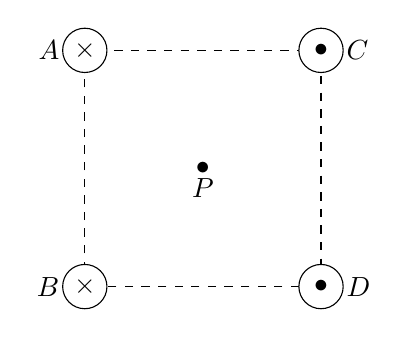
\begin{tikzpicture}
			\coordinate[label=below:$P$] (P) at (1.5,1.5);
			\coordinate[label=left:$A$] (A) at (-.2,3);
			\coordinate[label=left:$B$] (B) at (-.2,0);
			\coordinate[label=right:$C$] (C) at (3.2,3);
			\coordinate[label=right:$D$] (D) at (3.2,0);
			\draw[dashed] (0,0) rectangle (3,3);
			\filldraw[fill=white] (0,0) circle (8pt) node {$\times$};
			\filldraw[fill=white] (0,3) circle (8pt) node {$\times$};
			\filldraw[fill=white] (3,3) circle (8pt) node {$\bullet$};
			\filldraw[fill=white] (3,0) circle (8pt) node {$\bullet$};
			\node at (P) {$\bullet$};
		\end{tikzpicture}
	\end{figure}
	\item ខ្សែចម្លងវែងប្រវែងអនន្តពីរត្រូវបានដាក់ស្របគ្នា ស្ថិតនៅចម្ងាយ $d=20\si{\centi\metre}$ ពីគ្នា។ ខ្សែចម្លងទាំងពីរឆ្លងកាត់ដោយចរន្ត $I_{1}=3.0\si{\ampere}$ និង $I_{2}=5.0\si{\ampere}$ មានទិសដៅដូចគ្នា ដូចបង្ហាញក្នុងរូប។
	\begin{enumerate}
		\item គណនាដែនម៉ាញេទិចផ្គូបត្រង់ចំណុចកណ្តាលនៃខ្សែចម្លងទាំងពីរ។
		\item គណនាដែនម៉ាញេទិចផ្គួបត្រង់ចំណុច $P$ ដែលស្ថិតនៅចម្ងាយ $d=20\si{\centi\meter}$ ពីខ្សែទី២។
		\begin{figure}[H]
			\centering
			\begin{tikzpicture}
				\coordinate (O) at (0,0);
				\coordinate (I) at (3,0);
				\coordinate[label=below:{$d$}] (d1) at (1.5,-.1);
				\coordinate[label=left:{$d$}] (d2) at (3,1.5);
				\coordinate[label=above:{$P$}] (P) at (3,3);
				\draw[dashed, black] (O) to (I);
				\draw[dashed, black] (I) to (P);
				\node at (P) {$\bullet$};
				\coordinate[label=left:{$I_{1}$}] (I1) at (-.2,0);
				\coordinate[label=right:{$I_{2}$}] (I2) at (3.2,0);
				\filldraw[fill=white] (O) circle (8pt) node {$\bullet$};
				\filldraw[fill=white] (I) circle (8pt) node {$\bullet$};
				\draw[->] (1.7,-.5) to (3,-.5);
				\draw[<-] (0,-.5) to (1.3,-.5);
				\draw[->] (2.7,1.7) to (2.7,3);
				\draw[<-] (2.7,.3) to (2.7,1.3);
			\end{tikzpicture}
		\end{figure}
	\end{enumerate}
	\item ខ្សែចម្លងវង់មួយមានកាំ $R=5\si{\centi\metre}$ ឆ្លងកាត់ដោយចរន្ត $I=5\si{\ampere}$។ រង្វង់ខ្សែត្រូវបានដាក់ក្នុងដែនម៉ាញេទិចឯកសណ្ឋានដែលមានអាំងឌុចស្យុង $B=8\times10^{-5}\si{\tesla}$។\\ កំណត់ដែនម៉ាញេទិចផ្គួបត្រង់ផ្ចិត $O$ នៃរង្វង់ខ្សែត្រូវបានដាក់ឲ្យស្របនឹងខ្សែដែនម៉ាញេទិច។
\end{enumerate}
